%======================================================================
\NEWSEC
%======================================================================

\subsection{\ssParticles}

\begin{frame}[fragile,label=ss-particles] 
\secframetitle{\ssParticles}
\greenbf{Particle classes represent particle data on \code{Block}s}
\ \\
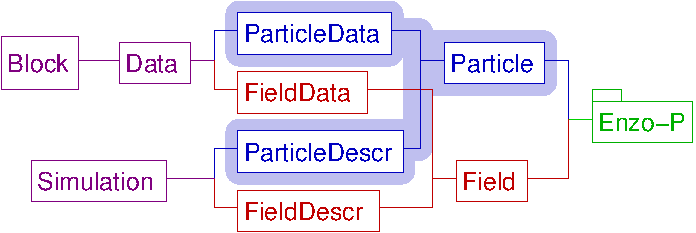
\includegraphics[width=2in]{data-classes-particle.pdf}

\begin{itemize}
\item \greencode{ParticleBlock}
\begin{itemize}
\item represents state-independent (intrinsic) data
\item associated with \greencode{Block}'s: one per mesh node
\item raw arrays
\end{itemize}
\item \greencode{ParticleDescr}
\begin{itemize}
\item represents state-dependent (extrinsic) data
\item associated with \greencode{Simulation} object: one per process
\end{itemize}
\item Applications access particle data via \greencode{Particle} objects
\end{itemize}
\end{frame}

%----------------------------------------------------------------------

\begin{frame}[fragile,label=ss-particles] 
\secframetitle{\ssParticles}
\greenbf{Particle classes represent particle data on \code{Block}s}
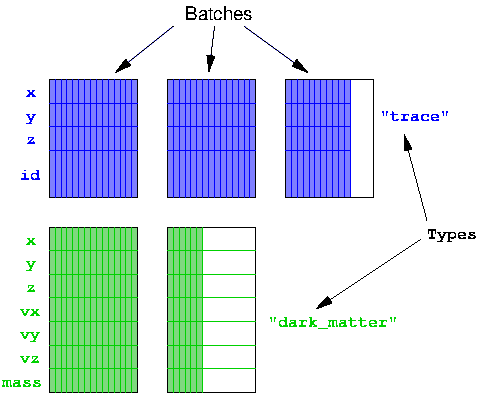
\includegraphics[width=2.0in]{particles-design.pdf} \ \\
\end{frame}

